\subsection{Specification}\hypertarget{home}{}
\paragraph{Model 1} (Pseudo Poisson)
\begin{equation*}
    \begin{split}
        y_{it}&=x_{it1}^{\beta_1}x_{it2}^{\beta_2}x_{it3}^{\beta_3}\theta_i\epsilon_{it}\\
        &= f(x_{it};\beta)\theta_i\epsilon_{it}\\
    \end{split}
\end{equation*}

Tables: \hyperlink{reg_inf_pois_2022}{Pois}

\paragraph{Reference} to Koen Jochman's lecture notes on panel data and model with multiplicative
effect:
\begin{equation*}
    y_{it}=f(x_{it};\beta)\theta_i\epsilon_{it} \quad \text{where} \quad \E\bra{\epsilon_{it}|x_{i1},\ldots,x_{iT},\theta_i}=1
\end{equation*}
Then following the same logic in additive effect, we difference out individual effect to get:
\begin{equation*}
    \E\bra{\frac{y_{it}}{f(x_{it};\beta)}-\frac{y_{i,t-1}}{f(x_{i,t-1};\beta)}\bigg | x_{i1},\ldots,x_{iT}}=0
\end{equation*}
Similarly, \begin{equation*}
    \E\bra{\frac{y_{it}}{f(x_{it};\beta)}-\frac{\sum_{t=1}y_{it}}{\sum_{t=1}f(x_{it};\beta)}\bigg | x_{i1},\ldots,x_{iT}}=0
\end{equation*}
One of the unconditional moment equation given rise to is \begin{equation}
    \E\bra{x_it\pa{\frac{y_{it}}{f(x_{it};\beta)}-\frac{\sum_{t=1}y_{it}}{\sum_{t=1}f(x_{it};\beta)}}}=0
\end{equation}
The moment conditon is often called pseudo-poisson estimator (as if assuming $y_it|x_{i1},\ldots,x_{iT},\theta_i\sim Poisson(f(x_{it};\beta)\theta_i)$ and then use maximum likelihood.)
When regressors are not strictly exogenous, we can construct a \textbf{differencing} based estimator based on sequential moment restrictions.
The \verb+fixest+ package doesn't provide the differencing based estimator. \\
\textbf{TO BE CONSTRUCTED BY HAND LATER.}

\begin{example}
    Consider a simple multiplicative error term model where \begin{equation*}
        y_{it}=\alpha_i f(x_{it};\beta)\epsilon_{it}
    \end{equation*}
    \begin{enumerate}
        \item If $\epsilon|\alpha_i,x_{it}\sim \calp(1)$, then we have \begin{equation*}
                  y_{it} | \alpha_i,\pa{m_{it}= f(x_{it};\beta)}\sim \calp(\alpha_i m_{it}) \to \E\bra{y_{it}|\alpha_i,x_{it}}=\alpha_i m_{it}
              \end{equation*}
        \item If $\log(\epsilon)|\alpha_i,x_{it}\sim \caln(0,\sigma^2)$, as long as
              $\E\bra{\epsilon_{it}|\alpha_i,x_{it}}=1$, we have \begin{equation*}
                  \E\bra{y_{it} | \alpha_i,m_{it}}=\alpha_i m_{it}
              \end{equation*}
    \end{enumerate}
    Consider an additive error term model where \begin{equation*}
        y_{it} = \alpha_i f(x_{it};\beta)+u_{it}
    \end{equation*} with $\E\bra{u_{it}|\alpha_i, m_{it}}=0$ we have the same conditional mean function $\E\bra{y_{it}|\alpha_i,m_{it}}=\alpha_i m_{it}$

\end{example}

\begin{remark}
    If we assume that $\epsilon_{it}$ is independent of $x_{it}$ and $\theta_i$, then \begin{equation*}
        \log(y_{it})=\log(f(x_{it};\beta))+\log(\theta_i)+\log(\epsilon_{it})
    \end{equation*}
    with $\E\bra{\log(\epsilon_{it})|x_{it},\theta_i}=\E\bra{\log(\epsilon_{it})}\neq \log\E\bra{\epsilon_{it}}$
\end{remark}

\paragraph{Model 2} (OLS)
\begin{align*}
    \log(y_{it}) & =\log(x_{it1})\beta_1+\log(x_{it2})\beta_2+\log(x_{it3})\beta_3+\log(\theta_i)+\log(\epsilon_{it}) \\
\end{align*}
LHS: log(ETP INF); \\ RHS: log(STAC INPATIENT), log(STAC OUTPATIENT),
log(SESSION),CASEMIX
\\Table: \hyperlink{reg_inf_ols_2022}{OLS},
\hyperlink{reg_inf_lag_2022}{OLS\_lag1}
\\Figure: \hyperlink{FE_OLS_FI}{FixedEffect\_OLS}

% \begin{remark}
%     The Pseudo poisson and Log OLS are equivalent if we assume that $\epsilon_{it}$ is independent of $x_{it}$ and $\theta_i$.
% \end{remark}

\begin{remark}
    The Mundlak (1978) approach is to include the average of the individual-specific variables $\bar{x_i}$ in the regression. He shows that it is equivalent to within group estimator.
    (Correlated random effect $\sim$ WG estimator). If the true model is \begin{equation*}
        y_{it}=x_{it}\beta+\theta_i+\epsilon_{it}
    \end{equation*} and $E(\theta_i|\bar{x}_i)=\bar{x}_i\gamma+\tilde{\theta}_i$, then
    \begin{equation*}
        y_{it}=(x_{it}-\bar{x}_i)\beta+\bar{x}_i(\gamma+\beta)+\tilde{\theta}_i+\epsilon_{it}
        (x_{it}-\bar{x}_i)\beta_1+\bar{x}_i\beta_2+\tilde{\theta}_i+\epsilon_{it}
    \end{equation*}
    Only when the $\theta_i$ is uncorrelated with $x_{it}$, the $\beta_1 = \beta_2$.
\end{remark}

\hypertarget{reg_inf_pois_2022}{Pois}

\begingroup
\centering
\begin{tabular}{lcc}
   \tabularnewline \midrule \midrule
   Dependent Variable: & \multicolumn{2}{c}{ETP\_INF}\\
   Model:              & (1)         & (2)\\  
   \midrule
   \emph{Variables}\\
   log(SEJHC\_MCO)     & 0.158$^{a}$ & 0.727$^{a}$\\   
                       & (0.028)     & (0.026)\\   
   log(SEJHP\_MCO)     & 0.044$^{a}$ & 0.107$^{a}$\\   
                       & (0.011)     & (0.019)\\   
   log(SEANCES\_MED)   & 0.032$^{a}$ & 0.043$^{a}$\\   
                       & (0.008)     & (0.011)\\   
   CASEMIX             & 0.007$^{a}$ & 0.014$^{a}$\\   
                       & (0.002)     & (0.003)\\   
   \midrule
   \emph{Fixed-effects}\\
   FI                  & Yes         & \\  
   FI\_EJ              &             & Yes\\  
   \midrule
   \emph{Fit statistics}\\
   Observations        & 3,928       & 3,928\\  
   Squared Correlation & 0.995       & 0.983\\  
   Pseudo R$^2$        & 0.966       & 0.956\\  
   \midrule \midrule
   \multicolumn{3}{l}{\emph{Signif. Codes: a: 0.01, b: 0.05, c: 0.1}}\\
\end{tabular}
\par\endgroup



\hyperlink{home}{Back}
\bigskip

\newpage
\hypertarget{reg_inf_ols_2022}{OLS}

\begingroup
\centering
\begin{tabular}{lcc}
   \tabularnewline \midrule \midrule
   Dependent Variable: & \multicolumn{2}{c}{log(ETP\_INF)}\\
   Model:              & (1)         & (2)\\  
   \midrule
   \emph{Variables}\\
   log(SEJHC\_MCO)     & 0.184$^{a}$ & 0.676$^{a}$\\   
                       & (0.026)     & (0.031)\\   
   log(SEJHP\_MCO)     & 0.032$^{a}$ & 0.097$^{a}$\\   
                       & (0.011)     & (0.022)\\   
   log(SEANCES\_MED)   & 0.021$^{a}$ & 0.037$^{a}$\\   
                       & (0.006)     & (0.010)\\   
   CASEMIX             & 0.007$^{b}$ & 0.013$^{a}$\\   
                       & (0.003)     & (0.004)\\   
   \midrule
   \emph{Fixed-effects}\\
   FI                  & Yes         & \\  
   FI\_EJ              &             & Yes\\  
   \midrule
   \emph{Fit statistics}\\
   Observations        & 3,923       & 3,923\\  
   Squared Correlation & 0.993       & 0.980\\  
   Pseudo R$^2$        & 1.77        & 1.39\\  
   \midrule \midrule
   \multicolumn{3}{l}{\emph{Signif. Codes: a: 0.01, b: 0.05, c: 0.1}}\\
\end{tabular}
\par\endgroup



\hyperlink{home}{Back}
\bigskip
\newpage
\hypertarget{reg_inf_lag_2022}{OLS\_lag1}

\begingroup
\centering
\begin{tabular}{lcc}
   \tabularnewline \midrule \midrule
   Dependent Variable: & \multicolumn{2}{c}{log(ETP\_INF)}\\
   Model:              & (1)         & (2)\\  
   \midrule
   \emph{Variables}\\
   log(SEJHC\_MCO)     & 0.222$^{a}$ & 0.692$^{a}$\\   
                       & (0.049)     & (0.036)\\   
   log(SEJHP\_MCO)     & 0.093$^{a}$ & 0.111$^{a}$\\   
                       & (0.025)     & (0.032)\\   
   log(SEANCES\_MED)   & 0.040$^{c}$ & 0.047$^{a}$\\   
                       & (0.023)     & (0.015)\\   
   CASEMIX             & 0.013$^{a}$ & 0.014$^{a}$\\   
                       & (0.003)     & (0.005)\\   
   \midrule
   \emph{Fixed-effects}\\
   FI                  & Yes         & \\  
   FI\_EJ              &             & Yes\\  
   \midrule
   \emph{Fit statistics}\\
   Observations        & 3,151       & 3,151\\  
   Squared Correlation & 0.994       & 0.983\\  
   Pseudo R$^2$        & 1.84        & 1.48\\  
   \midrule \midrule
   \multicolumn{3}{l}{\emph{Signif. Codes: a: 0.01, b: 0.05, c: 0.1}}\\
\end{tabular}
\par\endgroup



\hyperlink{home}{Back}
\bigskip
\newpage
\hypertarget{FE_OLS_FI}{FixedEffect\_OLS} Fixed effects extracted from OLS regression with fixed effect on each FI (not FI\_EJ).
\begin{figure}[!htbp]
    \centering
    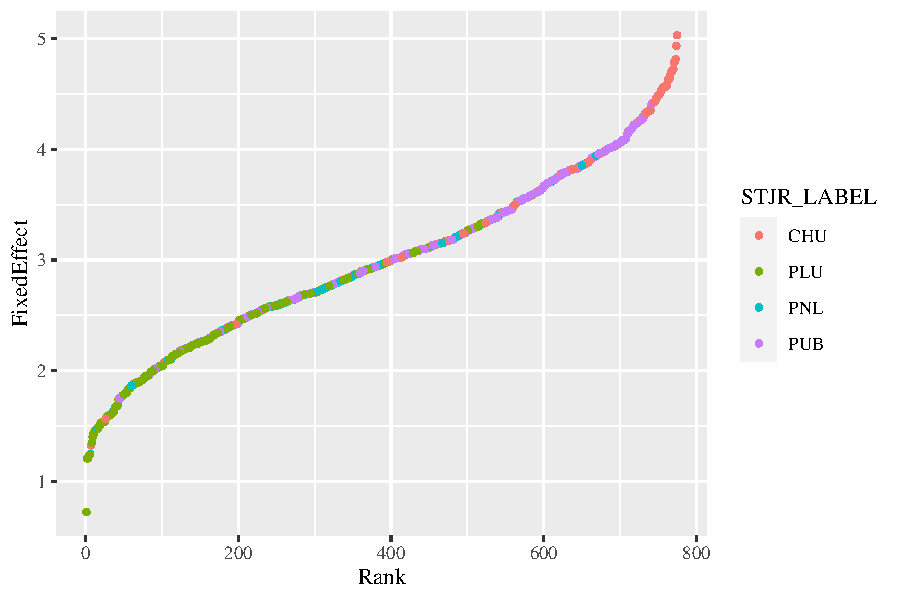
\includegraphics[width=0.8\textwidth]{../../Figures/2016-2022/FE_ols_FI.pdf}
    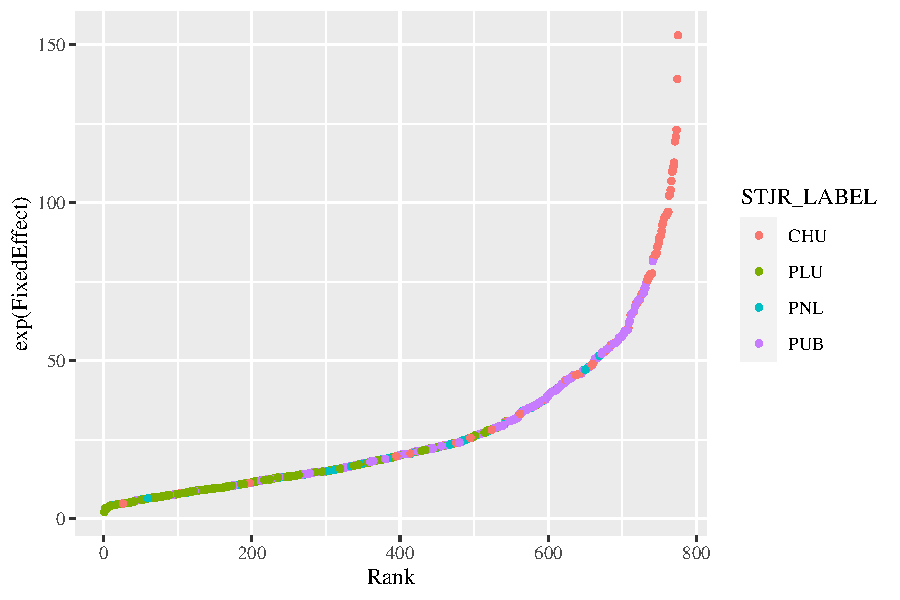
\includegraphics[width=0.8\textwidth]{../../Figures/2016-2022/FE_ols_FI_e.pdf}
\end{figure}
\hyperlink{home}{Back}
\bigskip